%für Sprache, A4 Blatt, float, Grafiken, UTF Codierung, PDF, Color, Seitenabstand, Listings
\documentclass[a4papr,12pt]{article}
\usepackage[utf8]{inputenc}
\usepackage[ngerman]{babel}
\usepackage{graphicx}
\usepackage{float}
\usepackage{textcomp}
\usepackage{pdfpages}
\usepackage{tikz}
\usepackage{hyperref}
\usepackage{geometry}
\usepackage{listings}
\usepackage{color}
\usepackage{booktabs}

%Mathematics
\usepackage{amstext}
\usepackage{amssymb}
\usepackage{amsmath}
\usepackage{amsfonts}
\usepackage{mathrsfs}
\usepackage{mathtools}

%include this before fancy or page style gets messed up bc of geometry
%Seitenabstand A4 Blatt
\geometry{a4paper}
\geometry{top=25mm,bottom=25mm,left=23mm,right=20mm}

% macro to select a scaled-down version of Bera Mono (for instance)
\makeatletter
\newcommand\BeraMonottfamily{%
  \def\fvm@Scale{0.85}% scales the font down
  \fontfamily{fvm}\selectfont% selects the Bera Mono font
}
\makeatother

%Hyperref zum anklicken von Überschriften in Texmaker + Farben einstellen
\hypersetup{
	colorlinks,
	citecolor=black,
	filecolor=black,
	linkcolor=blue,
	urlcolor=black
}

\definecolor{mygreen}{rgb}{0,0.6,0}
\definecolor{mygray}{rgb}{0.5,0.5,0.5}
\definecolor{mymauve}{rgb}{0.58,0,0.82}

%Zum Pascal Code einfügen mit lstinputlisting[language=Pascal] {../blabla.pas}
\lstset{ %
  backgroundcolor=\color{white},   % choose the background color; you must add \usepackage{color} or 								  \usepackage{xcolor}
  basicstyle=\BeraMonottfamily,        % the size of the fonts that are used for the code
  breakatwhitespace=false,         % sets if automatic breaks should only happen at whitespace
  breaklines=true,                 % sets automatic line breaking
  captionpos=b,                    % sets the caption-position to bottom
  commentstyle=\color{mygreen},    % comment style
  deletekeywords={...},            % if you want to delete keywords from the given language
  escapeinside={\%*}{*)},          % if you want to add LaTeX within your code
  extendedchars=true,              % lets you use non-ASCII characters; for 8-bits encodings only, 												does not work with UTF-8
  frame=single,	               % adds a frame around the code
  keepspaces=true,                 % keeps spaces in text, useful for keeping indentation of code 									  (possibly needs columns=flexible)
  keywordstyle=\color{blue},       % keyword style
  language=Octave,                 % the language of the code
  otherkeywords={...},           % if you want to add more keywords to the set
  numbers=left,                    % where to put the line-numbers; possible values are (none, left, 								  right)
  numbersep=5pt,                   % how far the line-numbers are from the code
  numberstyle=\tiny\color{black}, % the style that is used for the line-numbers
  rulecolor=\color{black},         % if not set, the frame-color may be changed on line-breaks within 								  not-black text (e.g. comments (green here))
  showspaces=false,                % show spaces everywhere adding particular underscores; it 														overrides 'showstringspaces'
  showstringspaces=false,          % underline spaces within strings only
  showtabs=false,                  % show tabs within strings adding particular underscores
  stepnumber=2,                    % the step between two line-numbers. If it's 1, each line will be 								  numbered
  stringstyle=\color{mymauve},     % string literal style
  title=\getlstname,
  tabsize=2,	                    % sets default tabsize to 2 spaces
  inputencoding=latin1,
  columns=fullflexible
}

\lstset{literate=%
	{Ö}{{\"O}}1
	{Ä}{{\"A}}1
	{Ü}{{\"U}}1
	{ß}{{\ss}}1
	{ü}{{\"u}}1
	{ä}{{\"a}}1
	{ö}{{\"o}}1
	{~}{{\textasciitilde}}1
}

%Filenamen und Pfad trennen
\makeatletter
\DeclareRobustCommand{\getlstname}{%
\begingroup
  % \lstname seems to change hyphens into \textendash
  \def\textendash{-}%
  \filename@parse{\lstname}%
  \texttt{\filename@base.\filename@ext}%
\endgroup
}


%Für Kopfzeile den Style
\usepackage{fancyhdr}
\pagestyle{fancy}
\lhead{1. Semester - Software Engineering}
\rhead{Andreas Roither, \today{}}

\begin{document}

%ANGABE 
%\thispagestyle{plain}
%\includepdf[pages={1},pagecommand={     
%\begin{tikzpicture}[remember picture, overlay]\node at (15.8, -1.35) {4 h};\end{tikzpicture}
%\begin{tikzpicture}[remember picture, overlay]\node at (7.6, -1.35) {Andreas Roither};\end{tikzpicture}
%\begin{Huge}
%\begin{tikzpicture}[remember picture, overlay]\node at (-1, -1.9) {X};\end{tikzpicture}
%\end{Huge}
%}]{Angabe/Uebung03.pdf}
%\includepdf[pages=2-,pagecommand={}]{testpdf}

% Makros fuer wahr/falsch in der Wahrheitstabelle:
\newcommand{\wahr}{\text{w}}
\newcommand{\falsch}{\text{f}}
% kann leicht geändert werden auf andere Darstellung, etwa mit 0 und 1:
%\newcommand{\wahr}{1}
%\newcommand{\falsch}{0}

\title{1. Semester - Software Engineering}
\author{Andreas Roither}
\date{bla{}, Hagenberg}
\maketitle
\newpage

\tableofcontents
\newpage


%LGI Übung%

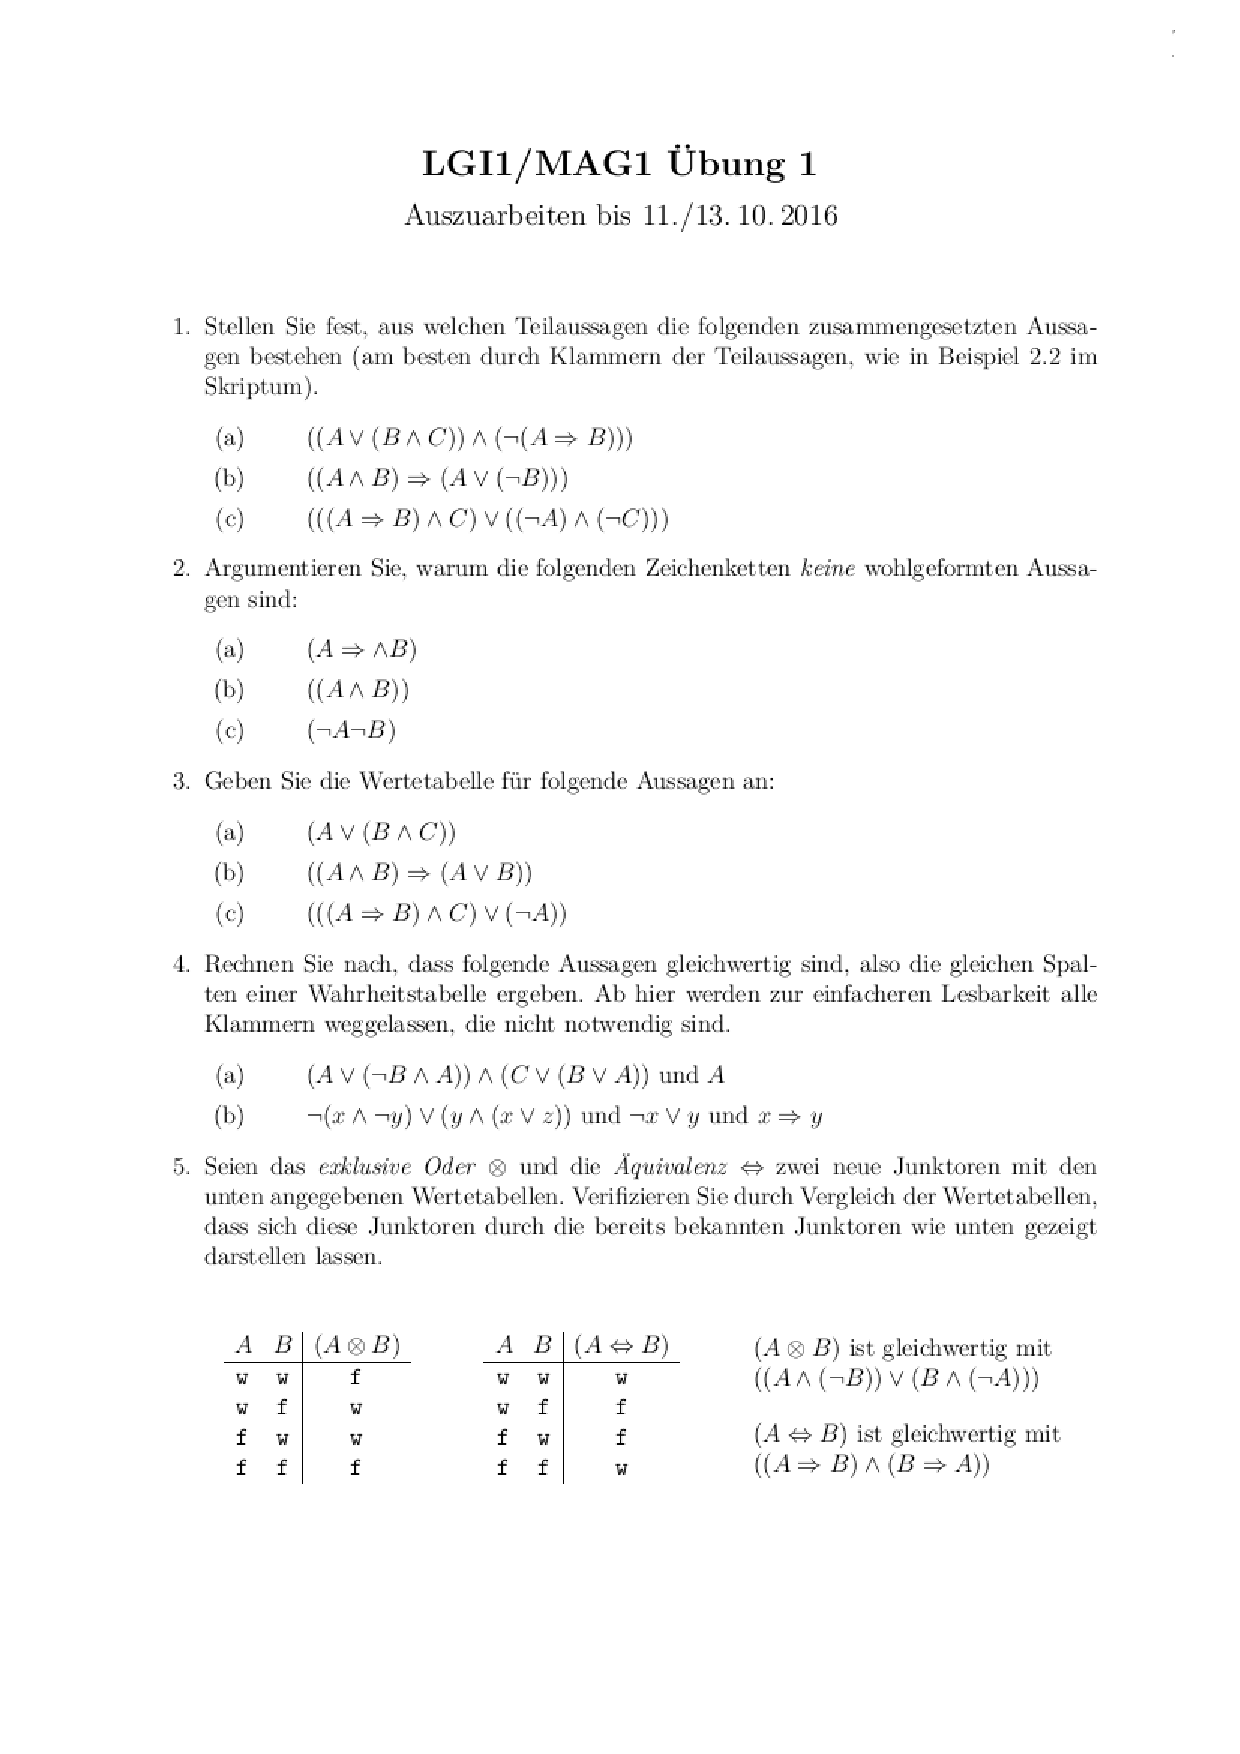
\includepdf[offset=-10 -45,pages=1,pagecommand={\section{LGI Übung} \subsection{Übung 1}}]{Angabe/LGI_Uebung01.pdf}
\includepdf[pages=2-,offset=-10 -45,pagecommand={}]{Angabe/LGI_Uebung01.pdf}
\begin{enumerate}
\item
\begin{enumerate}
\item $\conj{\disj{((A\lor\conj{(B\land C)}}\land\nega{(\neg \impl{(A \Rightarrow B)}))})}$
\item $\impl{(\conj{(A\land B)}\Rightarrow\disj{(A\lor\nega{(\neg B)}}))}$
\item $\disj{\conj{(\impl{(A\Rightarrow B)}\land C)} \conj{\nega{(\neg A)}\land\nega{(\neg C)}}}$
\end{enumerate}
\item
\begin{enumerate}
\item Aussage A endet mit Implikation (Junktor) -> nicht wohlgeformt
\item eine Klammer zu viel
\item es fehlen umhüllende Klammern
\end{enumerate}
\item 
\begin{enumerate}
\item Wahrheitstabelle

\begin{tabular}{|c|c|c|c|c|}
\hline
$A$ & $B$ & $C$ & $B \land C$ & $(A \lor (B \land C)))$\\ \hline
\falsch & \falsch 	& \falsch 	& \falsch	& \falsch	\\ \hline 
\falsch & \falsch 	& \wahr 	& \falsch 	& \falsch	\\ \hline 
\falsch & \wahr 	& \falsch 	& \falsch 	& \falsch	\\ \hline 
\falsch & \wahr 	& \wahr 	& \wahr 	& \wahr		\\ \hline 
\wahr 	& \falsch 	& \falsch 	& \falsch 	& \wahr		\\ \hline 
\wahr 	& \falsch 	& \wahr 	& \falsch 	& \wahr		\\ \hline 
\wahr 	& \wahr 	& \falsch 	& \falsch 	& \wahr		\\ \hline 
\wahr 	& \wahr 	& \wahr 	& \wahr 	& \wahr		\\ \hline 
\end{tabular}

\item Wahrheitstabelle \\
\begin{tabular}{|c|c|c|c|c|}
\hline
$A$ & $B$ & $A \land B$ & $A \lor B$ & $((A \land B) \Rightarrow (A \lor B))$\\ \hline
\falsch & \falsch 	& \falsch 	& \falsch	& \wahr		\\ \hline 
\falsch & \falsch 	& \falsch 	& \wahr 	& \wahr		\\ \hline 
\wahr 	& \wahr 	& \falsch 	& \wahr 	& \wahr		\\ \hline 
\wahr	& \wahr 	& \wahr 	& \wahr 	& \wahr		\\ \hline 
\end{tabular}
\\\\
Tautologie.. 	Wenn alle in einer Spalte Richtig sind\\
Widerspruch.. 	Wenn alle in einer Spalte Falsch sind

\item Wahrheitstabelle \\
\begin{tabular}{|c|c|c|c|c|c|}
\hline
$A$ & $B$ & $C$ & $(A \Rightarrow B)$ & $((A \Rightarrow B) \land C)$ & $((A \Rightarrow B)\land C) \lor(\neg A))$\\ \hline
\falsch & \falsch 	& \falsch 	& \wahr		& \falsch	& \wahr		\\ \hline 
\falsch & \falsch 	& \wahr 	& \wahr 	& \wahr		& \wahr		\\ \hline 
\falsch & \wahr 	& \falsch 	& \wahr 	& \falsch	& \wahr		\\ \hline 
\falsch & \wahr 	& \wahr 	& \wahr 	& \wahr		& \wahr		\\ \hline 
\wahr 	& \falsch 	& \falsch 	& \falsch 	& \falsch	& \falsch	\\ \hline 
\wahr 	& \falsch 	& \wahr 	& \falsch 	& \falsch	& \falsch	\\ \hline 
\wahr 	& \wahr 	& \falsch 	& \wahr 	& \falsch	& \falsch	\\ \hline 
\wahr 	& \wahr 	& \wahr 	& \wahr 	& \wahr		& \wahr		\\ \hline 
\end{tabular}
\end{enumerate}

\newpage
\item
\begin{enumerate}
\item Wahrheitstabelle\\
\begin{tabular}{|c|c|c|c|c|c|c|}
\hline
$A$ & $B$ & $C$ & $(A \lor(\neg B \land A))$ & $(C \lor (B \lor A))$ & $(1 \land 2)$ & $A$\\ \hline
\falsch & \falsch 	& \falsch 	& \falsch	& \falsch	& \falsch	& \falsch	\\ \hline 
\falsch & \falsch 	& \wahr 	& \falsch 	& \wahr		& \falsch	& \falsch	\\ \hline 
\falsch & \wahr 	& \falsch 	& \falsch 	& \wahr		& \falsch	& \falsch	\\ \hline 
\falsch & \wahr 	& \wahr 	& \falsch 	& \wahr		& \falsch	& \falsch	\\ \hline 
\wahr 	& \falsch 	& \falsch 	& \wahr 	& \wahr		& \wahr		& \wahr		\\ \hline 
\wahr 	& \falsch 	& \wahr 	& \wahr 	& \wahr		& \wahr		& \wahr		\\ \hline 
\wahr 	& \wahr 	& \falsch 	& \wahr 	& \wahr		& \wahr		& \wahr		\\ \hline 
\wahr 	& \wahr 	& \wahr 	& \wahr 	& \wahr		& \wahr		& \wahr		\\ \hline 
\end{tabular}
\\\\
Wenn zwei Spalten die selben Werte haben(wahr,falsch) dann sind diese Ident $\equiv$
\item Wahrheitstabelle\\
\begin{tabular}{|c|c|c|c|c|c|c|c|}
\hline
$x$ & $y$ & $z$ & $\neg(x\land \neg y)$ & $(y\land (x \lor z))$ & $(1 \lor 2)$ & $\neg x\lor y$ & $x\Rightarrow y$\\ \hline
\falsch & \falsch 	& \falsch 	& \wahr		& \falsch	& \wahr		& \wahr		& \wahr		\\ \hline 
\falsch & \falsch 	& \wahr 	& \wahr 	& \falsch	& \wahr		& \wahr		& \wahr		\\ \hline 
\falsch & \wahr 	& \falsch 	& \wahr 	& \falsch	& \wahr		& \wahr		& \wahr		\\ \hline 
\falsch & \wahr 	& \wahr 	& \wahr 	& \wahr		& \wahr		& \wahr		& \wahr		\\ \hline 
\wahr 	& \falsch 	& \falsch 	& \falsch 	& \falsch	& \falsch	& \falsch	& \falsch	\\ \hline 
\wahr 	& \falsch 	& \wahr 	& \falsch 	& \falsch	& \falsch	& \falsch	& \falsch	\\ \hline 
\wahr 	& \wahr 	& \falsch 	& \wahr 	& \wahr		& \wahr		& \wahr		& \wahr		\\ \hline 
\wahr 	& \wahr 	& \wahr 	& \wahr 	& \wahr		& \wahr		& \wahr		& \wahr		\\ \hline 
\end{tabular}
\end{enumerate}
\item\begin{enumerate}
\item Wahrheitstabelle\\
\begin{tabular}{|c|c|c|c|c|c|}
\hline
$A$ & $B$ & $(A\land(\neg B))$ & $(B\land(\neg A))$ & $(1 \lor 2)$ & $A \otimes B$\\ \hline
\falsch & \falsch 	& \falsch	& \falsch	& \falsch	& \falsch	\\ \hline 
\falsch & \wahr 	& \falsch 	& \wahr		& \wahr		& \wahr		\\ \hline 
\wahr 	& \falsch 	& \wahr 	& \falsch	& \wahr		& \wahr		\\ \hline 
\wahr 	& \wahr 	& \falsch 	& \falsch	& \falsch	& \falsch	\\ \hline 
\end{tabular}
\\\\
Wenn zwei Spalten die selben Werte haben(wahr,falsch) dann sind diese Ident $\equiv$
\item Wahrheitstabelle\\
\begin{tabular}{|c|c|c|c|c|c|}
\hline
$A$ & $B$ & $(A\Rightarrow B))$ & $(B\Rightarrow A))$ & $(1 \land 2)$ & $A \iff B$\\ \hline
\falsch & \falsch 	& \wahr		& \wahr		& \wahr		& \wahr		\\ \hline 
\falsch & \wahr 	& \wahr 	& \falsch	& \falsch	& \falsch	\\ \hline 
\wahr 	& \falsch 	& \falsch 	& \wahr		& \falsch	& \falsch	\\ \hline 
\wahr 	& \wahr 	& \wahr 	& \wahr		& \wahr		& \wahr		\\ \hline 
\end{tabular}
\end{enumerate}
\item $2^n$ bei zweistelligen Junktoren $2^4$
\end{enumerate}


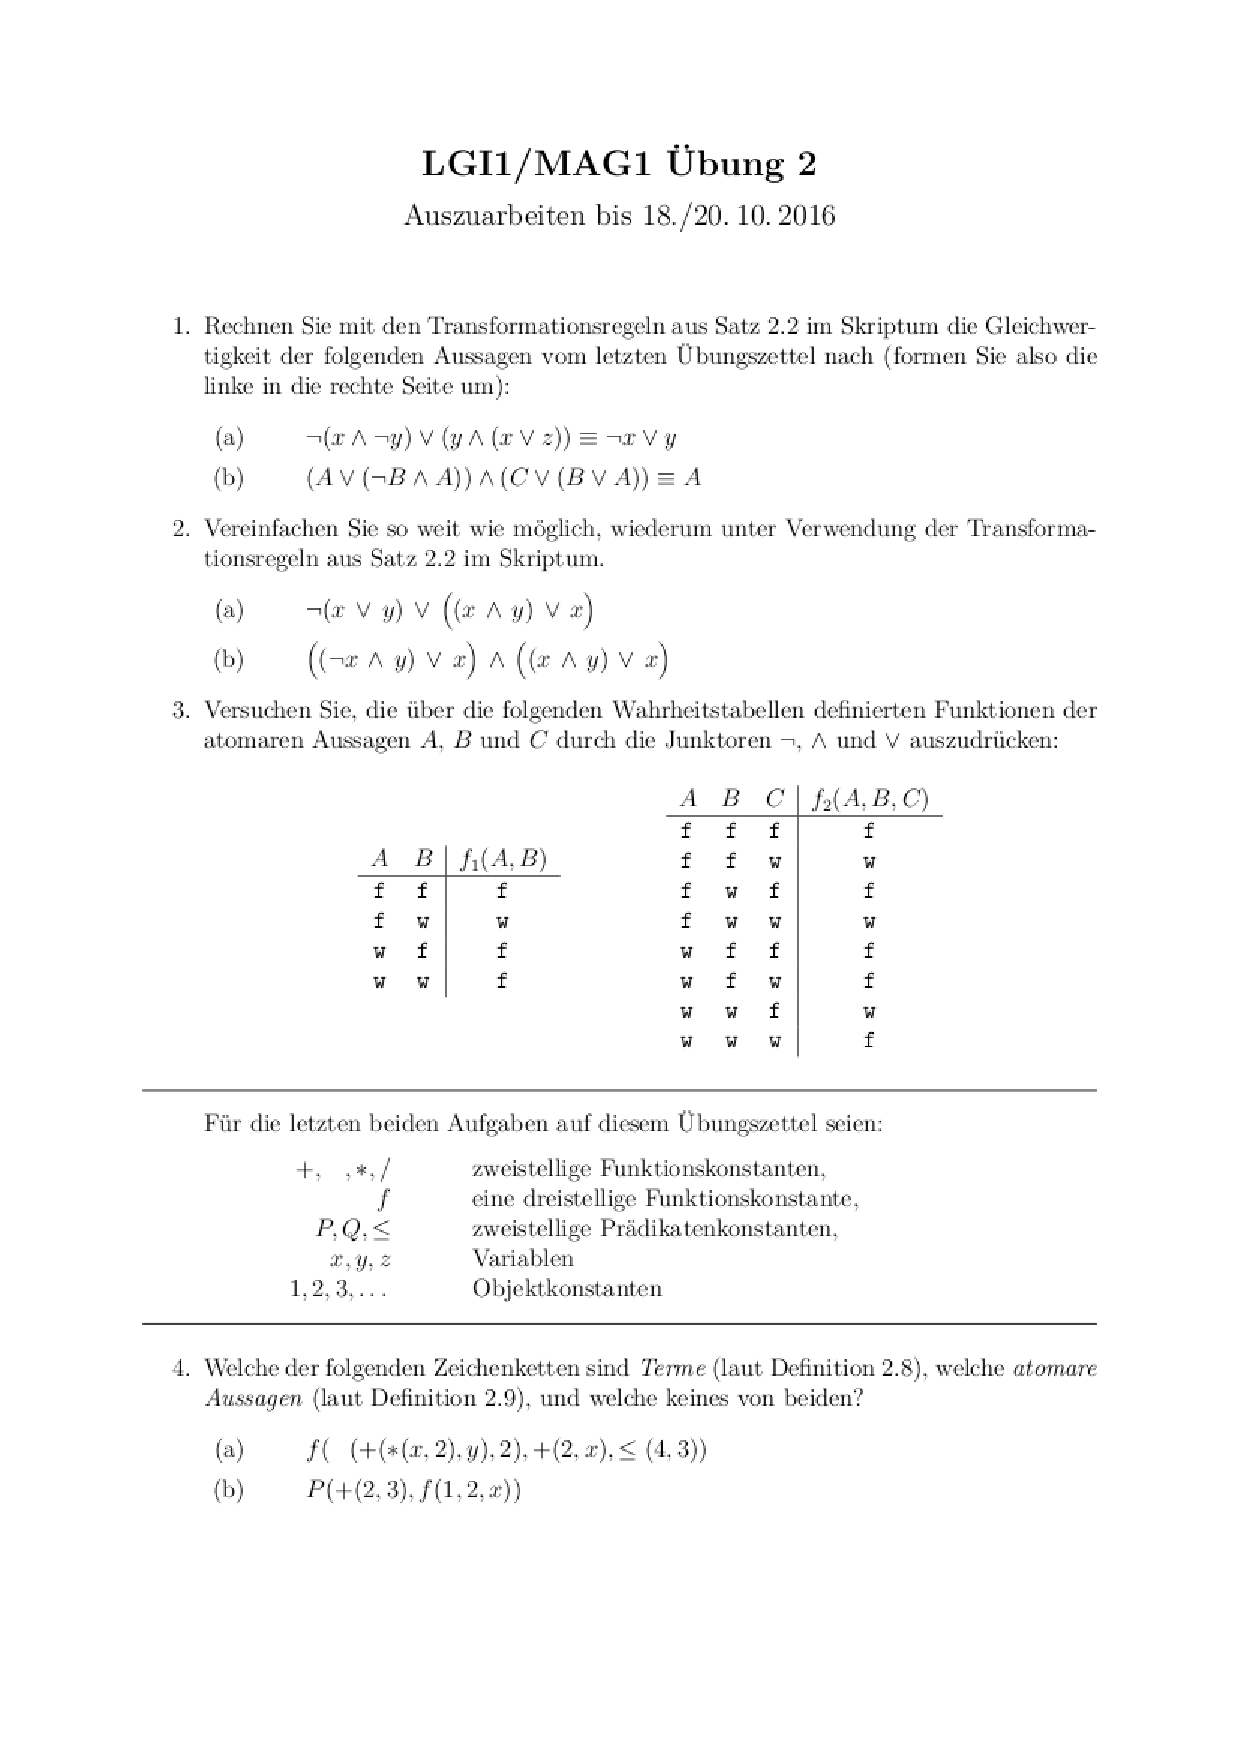
\includepdf[offset=-10 -25,pages=1,pagecommand={\subsection{Übung 2}}]{Angabe/LGI_Uebung02.pdf}
\includepdf[pages=2-,offset=-10 -25,pagecommand={}]{Angabe/LGI_Uebung02.pdf}

test




\includepdf[offset=-10 -25,pages=1,pagecommand={\subsection{Übung 3}}]{Angabe/LGI_Uebung03.pdf}

\includepdf[pages=2-,offset=-10 -25,pagecommand={}]{Angabe/LGI_Uebung03.pdf}

test

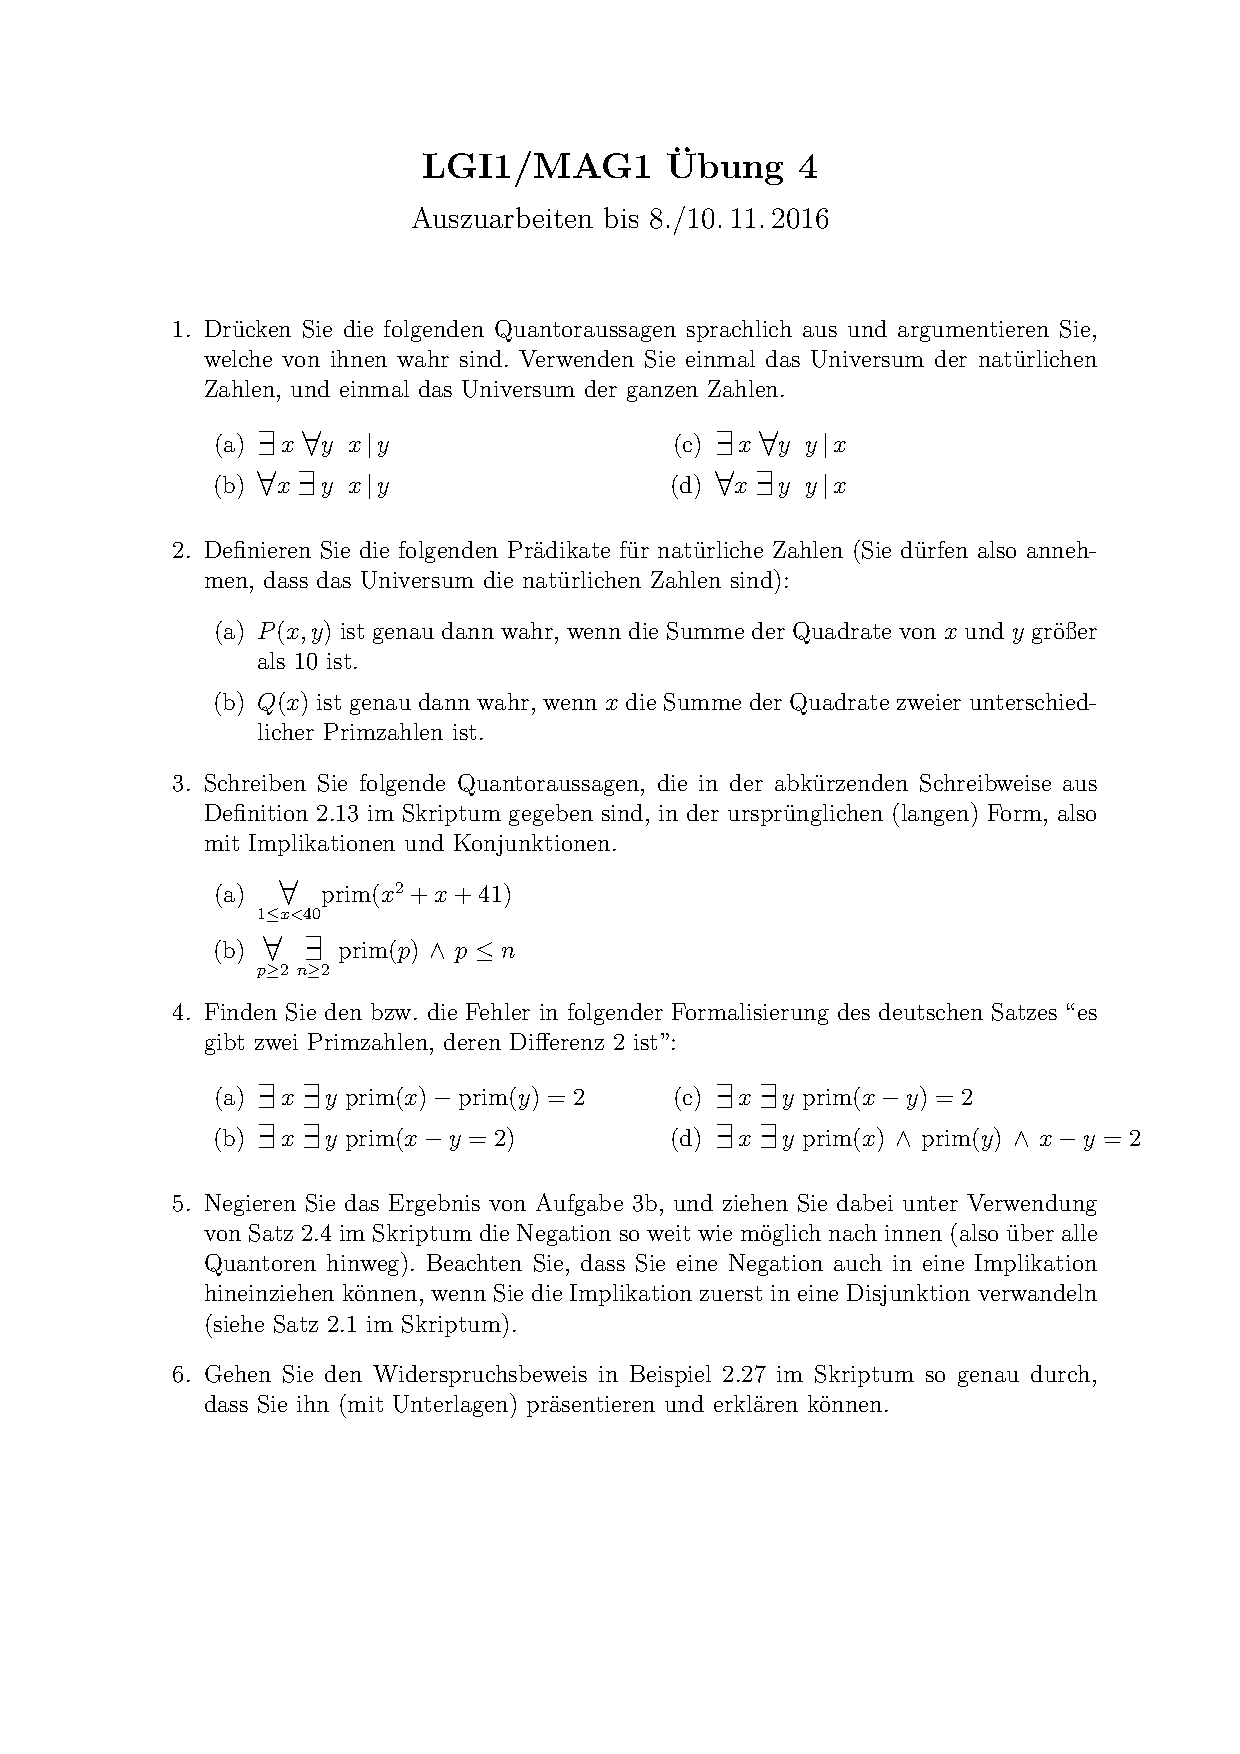
\includepdf[offset=-10 -25,pages=1,pagecommand={\subsection{Übung 4}}]{Angabe/LGI_Uebung04.pdf}

test

%EIR Übung%

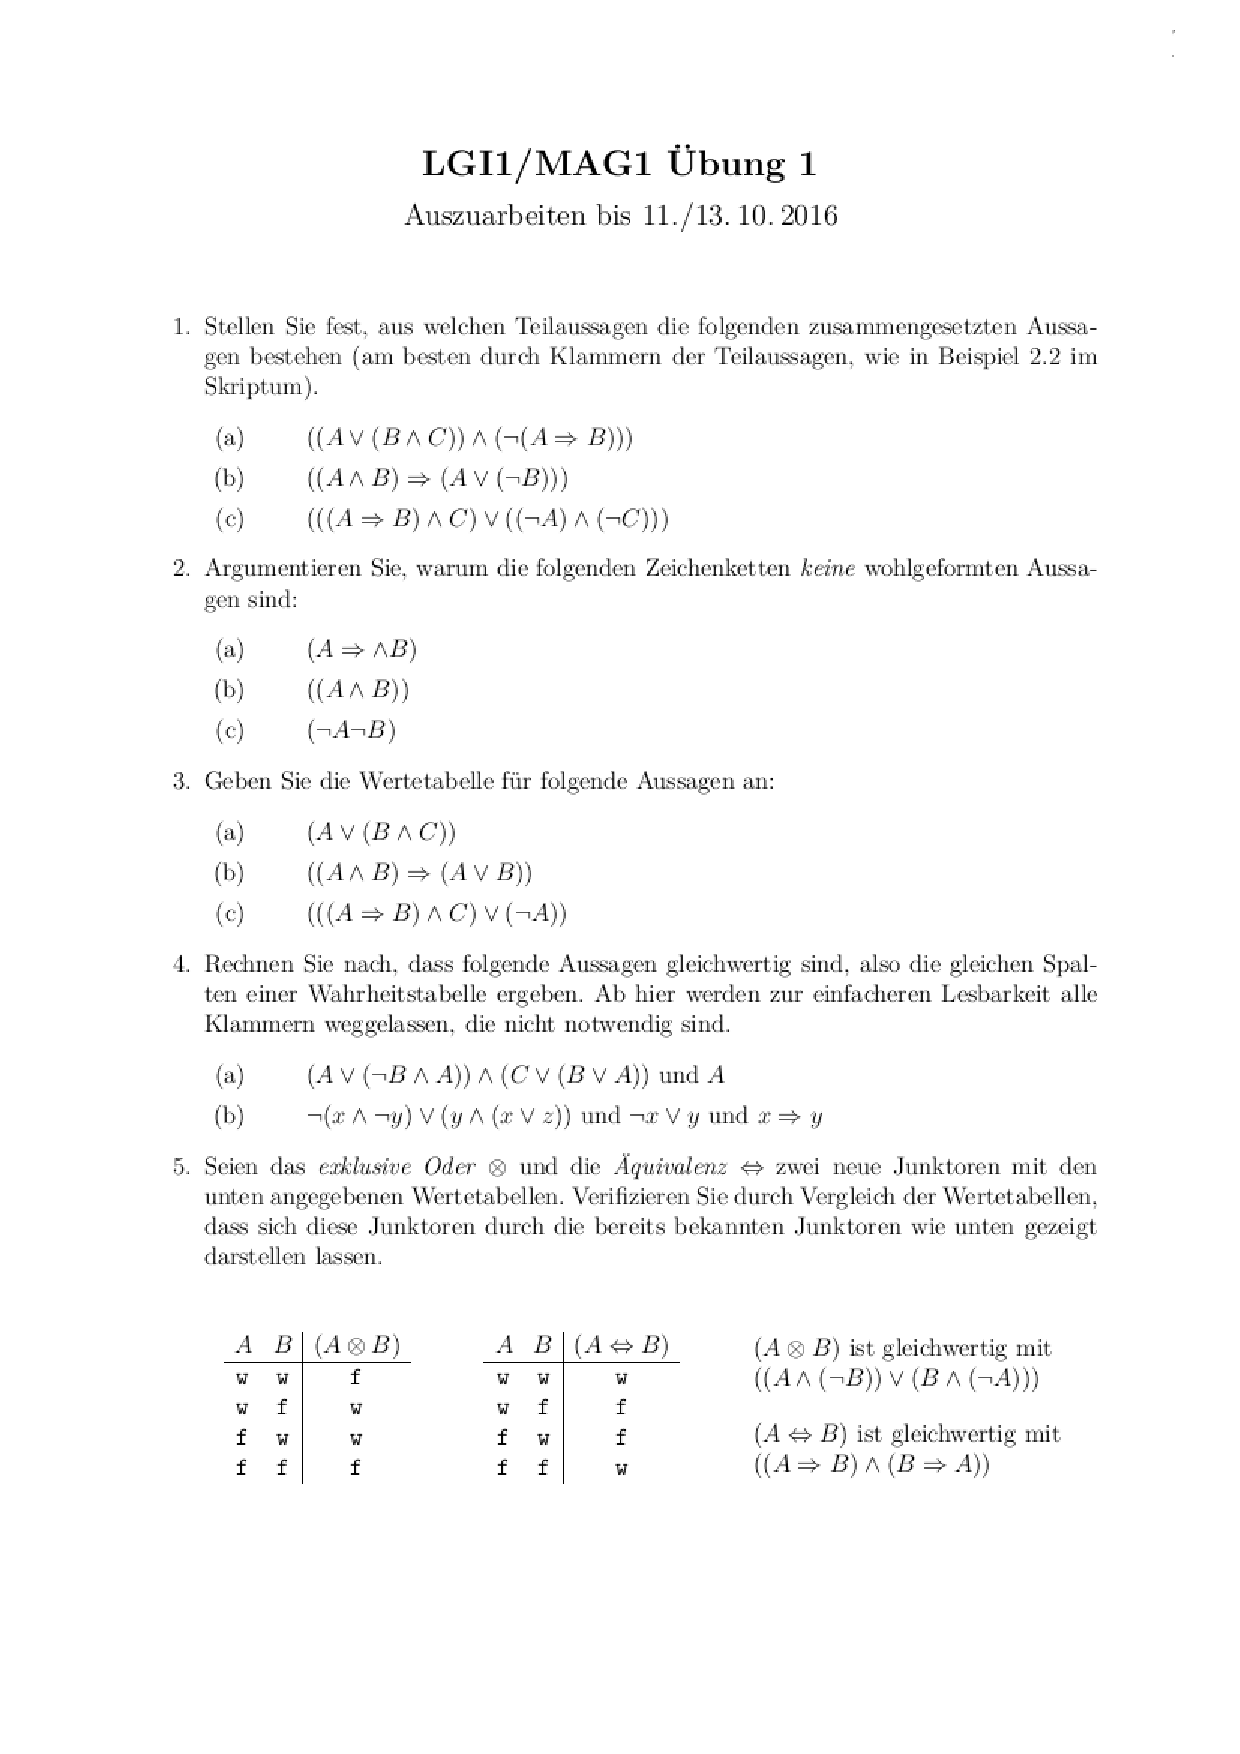
\includepdf[offset=-10 -45,pages=1,pagecommand={\section{EIR Übung} \subsection{Übung 1}}]{Angabe/LGI_Uebung01.pdf}
\includepdf[pages=2-,offset=-10 -45,pagecommand={}]{Angabe/LGI_Uebung01.pdf}
\begin{enumerate}
\item
\begin{enumerate}
\item $\conj{\disj{((A\lor\conj{(B\land C)}}\land\nega{(\neg \impl{(A \Rightarrow B)}))})}$
\item $\impl{(\conj{(A\land B)}\Rightarrow\disj{(A\lor\nega{(\neg B)}}))}$
\item $\disj{\conj{(\impl{(A\Rightarrow B)}\land C)} \conj{\nega{(\neg A)}\land\nega{(\neg C)}}}$
\end{enumerate}
\item
\begin{enumerate}
\item Aussage A endet mit Implikation (Junktor) -> nicht wohlgeformt
\item eine Klammer zu viel
\item es fehlen umhüllende Klammern
\end{enumerate}
\item 
\begin{enumerate}
\item Wahrheitstabelle

\begin{tabular}{|c|c|c|c|c|}
\hline
$A$ & $B$ & $C$ & $B \land C$ & $(A \lor (B \land C)))$\\ \hline
\falsch & \falsch 	& \falsch 	& \falsch	& \falsch	\\ \hline 
\falsch & \falsch 	& \wahr 	& \falsch 	& \falsch	\\ \hline 
\falsch & \wahr 	& \falsch 	& \falsch 	& \falsch	\\ \hline 
\falsch & \wahr 	& \wahr 	& \wahr 	& \wahr		\\ \hline 
\wahr 	& \falsch 	& \falsch 	& \falsch 	& \wahr		\\ \hline 
\wahr 	& \falsch 	& \wahr 	& \falsch 	& \wahr		\\ \hline 
\wahr 	& \wahr 	& \falsch 	& \falsch 	& \wahr		\\ \hline 
\wahr 	& \wahr 	& \wahr 	& \wahr 	& \wahr		\\ \hline 
\end{tabular}

\item Wahrheitstabelle \\
\begin{tabular}{|c|c|c|c|c|}
\hline
$A$ & $B$ & $A \land B$ & $A \lor B$ & $((A \land B) \Rightarrow (A \lor B))$\\ \hline
\falsch & \falsch 	& \falsch 	& \falsch	& \wahr		\\ \hline 
\falsch & \falsch 	& \falsch 	& \wahr 	& \wahr		\\ \hline 
\wahr 	& \wahr 	& \falsch 	& \wahr 	& \wahr		\\ \hline 
\wahr	& \wahr 	& \wahr 	& \wahr 	& \wahr		\\ \hline 
\end{tabular}
\\\\
Tautologie.. 	Wenn alle in einer Spalte Richtig sind\\
Widerspruch.. 	Wenn alle in einer Spalte Falsch sind

\item Wahrheitstabelle \\
\begin{tabular}{|c|c|c|c|c|c|}
\hline
$A$ & $B$ & $C$ & $(A \Rightarrow B)$ & $((A \Rightarrow B) \land C)$ & $((A \Rightarrow B)\land C) \lor(\neg A))$\\ \hline
\falsch & \falsch 	& \falsch 	& \wahr		& \falsch	& \wahr		\\ \hline 
\falsch & \falsch 	& \wahr 	& \wahr 	& \wahr		& \wahr		\\ \hline 
\falsch & \wahr 	& \falsch 	& \wahr 	& \falsch	& \wahr		\\ \hline 
\falsch & \wahr 	& \wahr 	& \wahr 	& \wahr		& \wahr		\\ \hline 
\wahr 	& \falsch 	& \falsch 	& \falsch 	& \falsch	& \falsch	\\ \hline 
\wahr 	& \falsch 	& \wahr 	& \falsch 	& \falsch	& \falsch	\\ \hline 
\wahr 	& \wahr 	& \falsch 	& \wahr 	& \falsch	& \falsch	\\ \hline 
\wahr 	& \wahr 	& \wahr 	& \wahr 	& \wahr		& \wahr		\\ \hline 
\end{tabular}
\end{enumerate}

\newpage
\item
\begin{enumerate}
\item Wahrheitstabelle\\
\begin{tabular}{|c|c|c|c|c|c|c|}
\hline
$A$ & $B$ & $C$ & $(A \lor(\neg B \land A))$ & $(C \lor (B \lor A))$ & $(1 \land 2)$ & $A$\\ \hline
\falsch & \falsch 	& \falsch 	& \falsch	& \falsch	& \falsch	& \falsch	\\ \hline 
\falsch & \falsch 	& \wahr 	& \falsch 	& \wahr		& \falsch	& \falsch	\\ \hline 
\falsch & \wahr 	& \falsch 	& \falsch 	& \wahr		& \falsch	& \falsch	\\ \hline 
\falsch & \wahr 	& \wahr 	& \falsch 	& \wahr		& \falsch	& \falsch	\\ \hline 
\wahr 	& \falsch 	& \falsch 	& \wahr 	& \wahr		& \wahr		& \wahr		\\ \hline 
\wahr 	& \falsch 	& \wahr 	& \wahr 	& \wahr		& \wahr		& \wahr		\\ \hline 
\wahr 	& \wahr 	& \falsch 	& \wahr 	& \wahr		& \wahr		& \wahr		\\ \hline 
\wahr 	& \wahr 	& \wahr 	& \wahr 	& \wahr		& \wahr		& \wahr		\\ \hline 
\end{tabular}
\\\\
Wenn zwei Spalten die selben Werte haben(wahr,falsch) dann sind diese Ident $\equiv$
\item Wahrheitstabelle\\
\begin{tabular}{|c|c|c|c|c|c|c|c|}
\hline
$x$ & $y$ & $z$ & $\neg(x\land \neg y)$ & $(y\land (x \lor z))$ & $(1 \lor 2)$ & $\neg x\lor y$ & $x\Rightarrow y$\\ \hline
\falsch & \falsch 	& \falsch 	& \wahr		& \falsch	& \wahr		& \wahr		& \wahr		\\ \hline 
\falsch & \falsch 	& \wahr 	& \wahr 	& \falsch	& \wahr		& \wahr		& \wahr		\\ \hline 
\falsch & \wahr 	& \falsch 	& \wahr 	& \falsch	& \wahr		& \wahr		& \wahr		\\ \hline 
\falsch & \wahr 	& \wahr 	& \wahr 	& \wahr		& \wahr		& \wahr		& \wahr		\\ \hline 
\wahr 	& \falsch 	& \falsch 	& \falsch 	& \falsch	& \falsch	& \falsch	& \falsch	\\ \hline 
\wahr 	& \falsch 	& \wahr 	& \falsch 	& \falsch	& \falsch	& \falsch	& \falsch	\\ \hline 
\wahr 	& \wahr 	& \falsch 	& \wahr 	& \wahr		& \wahr		& \wahr		& \wahr		\\ \hline 
\wahr 	& \wahr 	& \wahr 	& \wahr 	& \wahr		& \wahr		& \wahr		& \wahr		\\ \hline 
\end{tabular}
\end{enumerate}
\item\begin{enumerate}
\item Wahrheitstabelle\\
\begin{tabular}{|c|c|c|c|c|c|}
\hline
$A$ & $B$ & $(A\land(\neg B))$ & $(B\land(\neg A))$ & $(1 \lor 2)$ & $A \otimes B$\\ \hline
\falsch & \falsch 	& \falsch	& \falsch	& \falsch	& \falsch	\\ \hline 
\falsch & \wahr 	& \falsch 	& \wahr		& \wahr		& \wahr		\\ \hline 
\wahr 	& \falsch 	& \wahr 	& \falsch	& \wahr		& \wahr		\\ \hline 
\wahr 	& \wahr 	& \falsch 	& \falsch	& \falsch	& \falsch	\\ \hline 
\end{tabular}
\\\\
Wenn zwei Spalten die selben Werte haben(wahr,falsch) dann sind diese Ident $\equiv$
\item Wahrheitstabelle\\
\begin{tabular}{|c|c|c|c|c|c|}
\hline
$A$ & $B$ & $(A\Rightarrow B))$ & $(B\Rightarrow A))$ & $(1 \land 2)$ & $A \iff B$\\ \hline
\falsch & \falsch 	& \wahr		& \wahr		& \wahr		& \wahr		\\ \hline 
\falsch & \wahr 	& \wahr 	& \falsch	& \falsch	& \falsch	\\ \hline 
\wahr 	& \falsch 	& \falsch 	& \wahr		& \falsch	& \falsch	\\ \hline 
\wahr 	& \wahr 	& \wahr 	& \wahr		& \wahr		& \wahr		\\ \hline 
\end{tabular}
\end{enumerate}
\item $2^n$ bei zweistelligen Junktoren $2^4$
\end{enumerate}

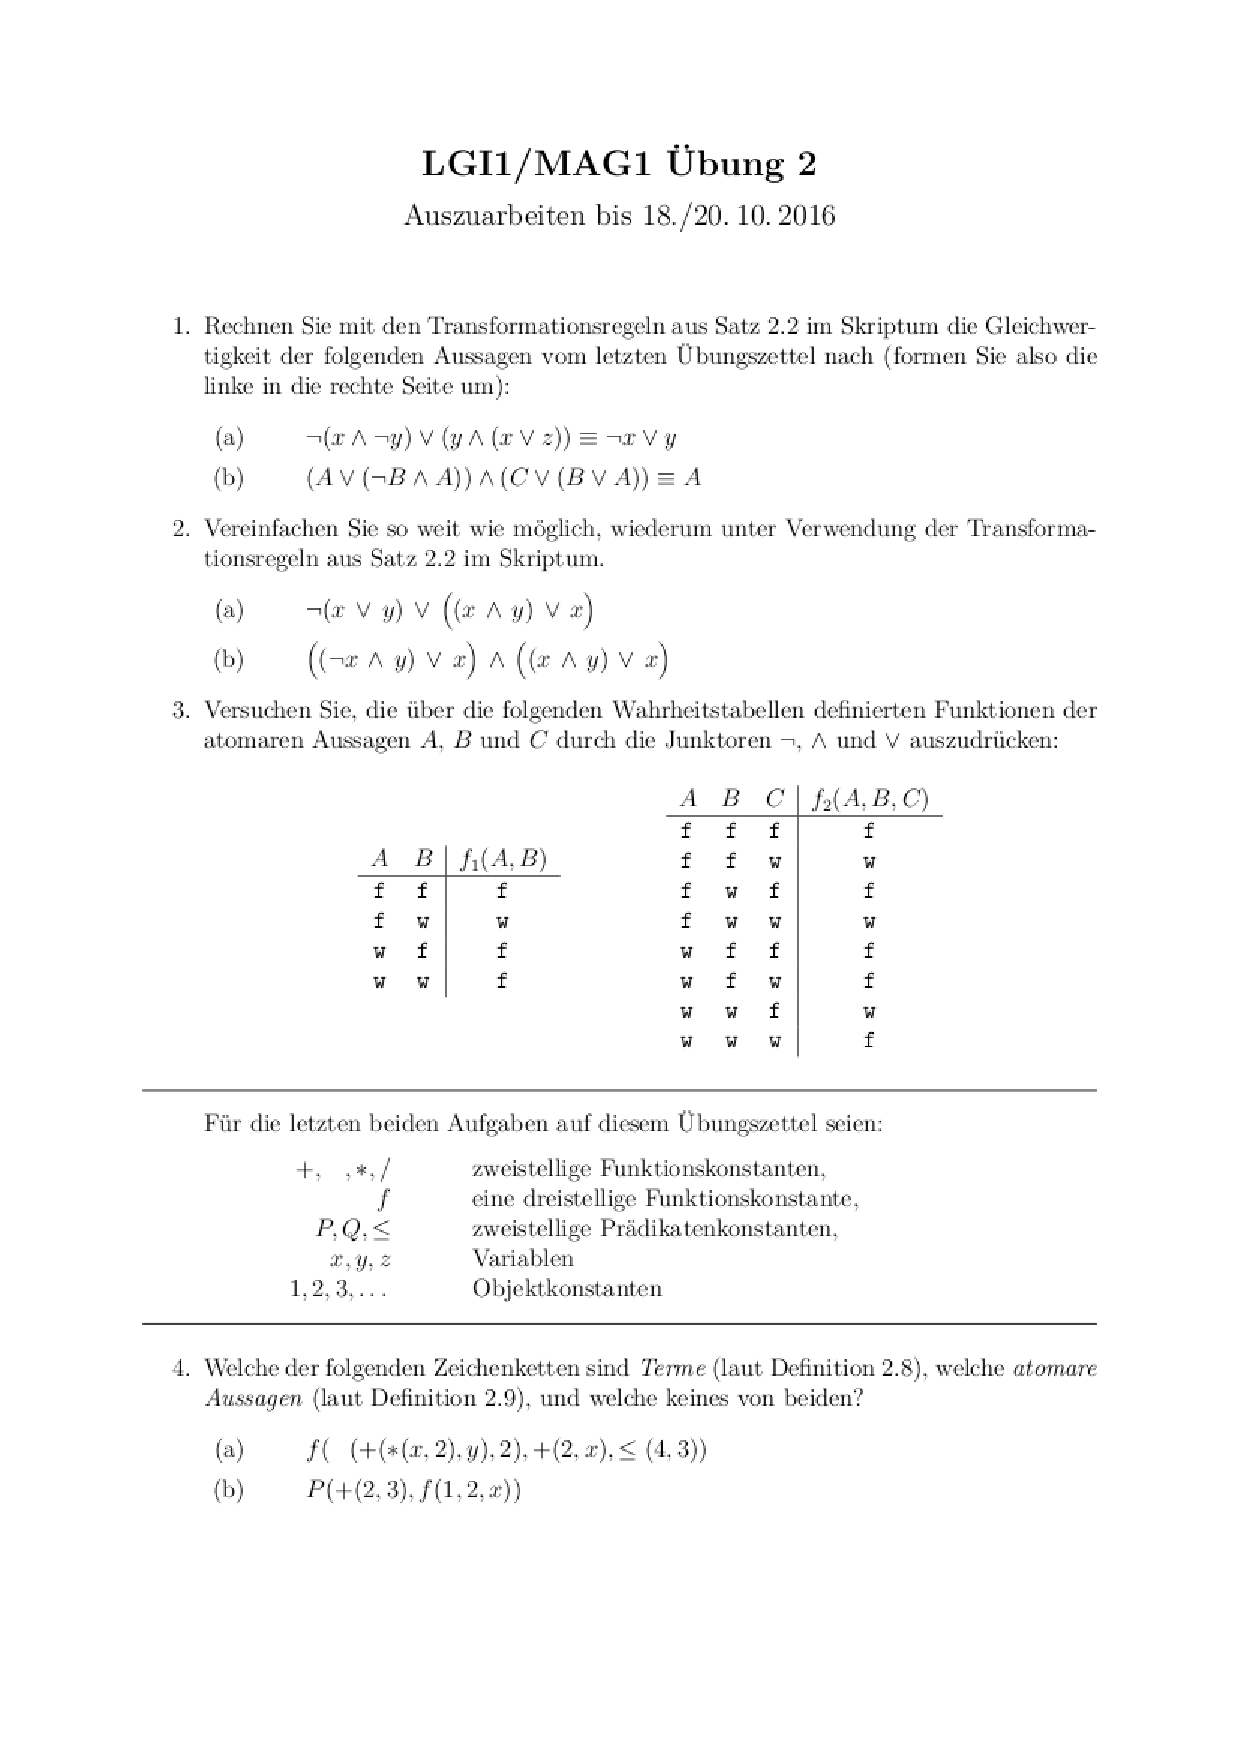
\includepdf[offset=-10 -25,pages=1,pagecommand={\subsection{Übung 2}}]{Angabe/LGI_Uebung02.pdf}
\includepdf[pages=2-,offset=-10 -25,pagecommand={}]{Angabe/LGI_Uebung02.pdf}

test


\includepdf[offset=-10 -25,pages=1,pagecommand={\subsection{Übung 3}}]{Angabe/LGI_Uebung03.pdf}

\includepdf[pages=2-,offset=-10 -25,pagecommand={}]{Angabe/LGI_Uebung03.pdf}

test



\end{document}





